\documentclass[12pt]{article}
\usepackage[paper=letterpaper,margin=2cm]{geometry}
\usepackage{amsmath}
\usepackage{amssymb}
\usepackage{amsfonts}
\usepackage{newtxtext, newtxmath}
\usepackage{enumitem}
\usepackage{titling}
\usepackage[colorlinks=true]{hyperref}
\usepackage{graphicx}
\usepackage{csvsimple}
\usepackage{luacode}
\setlength{\droptitle}{-6em}

% Enter the specific assignment number and topic of that assignment below, and replace "Your Name" with your actual name.

\title{\textbf{COMP0078 Assignment 2}}
\author{Student Numbers: 21168615 \& 19004608 \\ }
\date{Dec 14, 2022}

\begin{document}
    \maketitle
\section{PART I}
\subsection{Kernel Perceptron}
\subsubsection{Experimental Results}

\begin{itemize}
    \item[1.] Basic Results:

    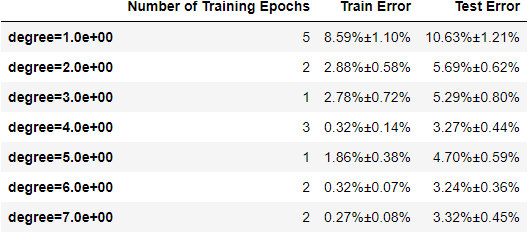
\includegraphics{outputs/part1/q1.png}


    \item[2.] Cross Validation Results:

    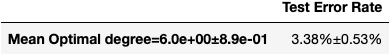
\includegraphics{outputs/part1/q2.png}

    \item[3.] Confusion Matrix:

    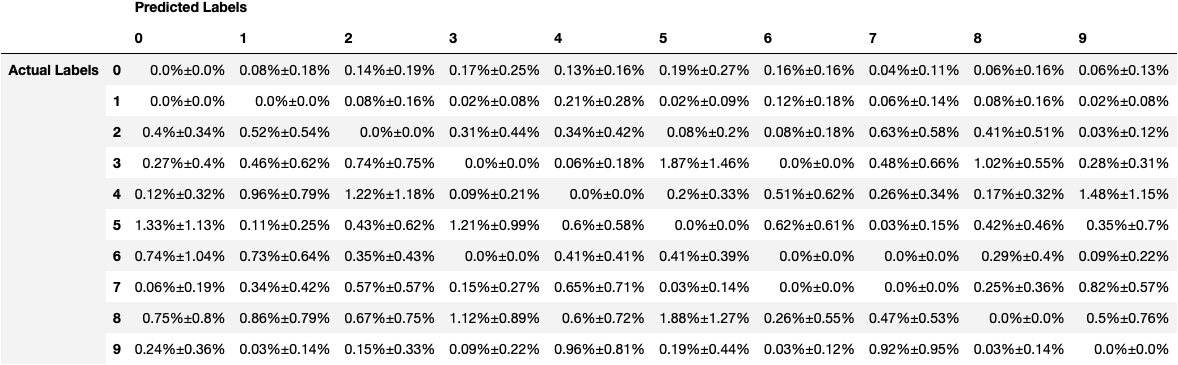
\includegraphics{outputs/part1/q3_confusion.png}
\newpage
    \item[4.] Hardest to predict images:

    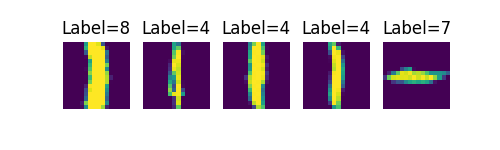
\includegraphics{outputs/part1/q4.png}
    \newpage
    \item[5.] Basic Results:

    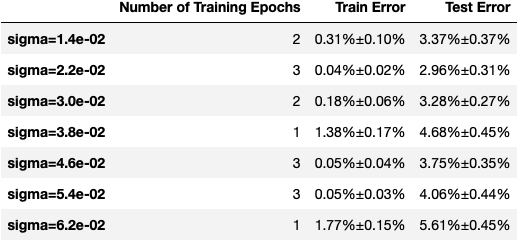
\includegraphics{outputs/part1/q5_1.png}

    Cross Validation Results:

    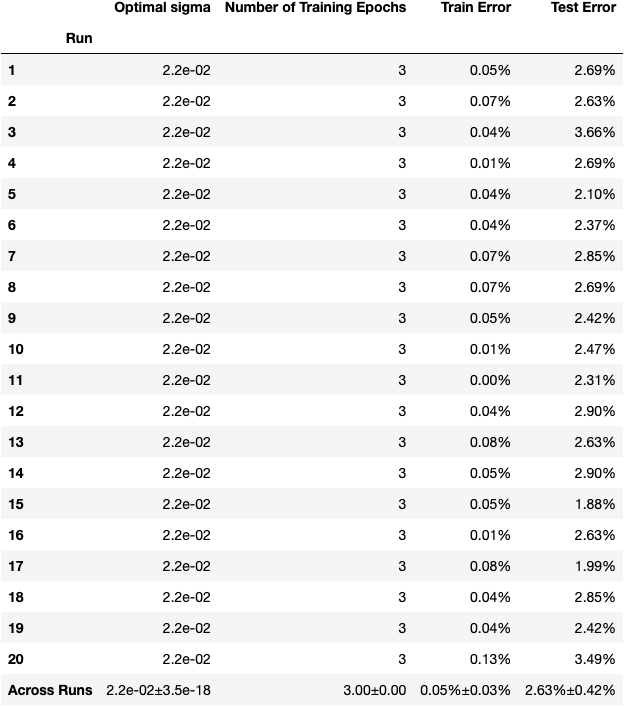
\includegraphics{outputs/part1/q5_2.png}
\end{itemize}
\subsubsection{Discussions}
    Choice of Parameters that weren't cross validated

    Generalisation to k-classifiers

    Kernel Comparison

    Kernel Perceptron Implementation


\newpage
\section{PART II}
\subsection{Semi-supervised Learning via Laplacian Interpolation}

Experimental report for the laplacian interpolation approach:
\\

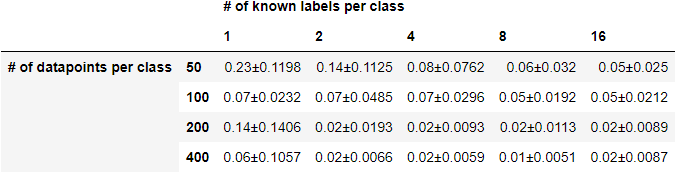
\includegraphics{outputs/part2/laplacian_interpolation_report.png}

\\

And for the laplacian kernel method:

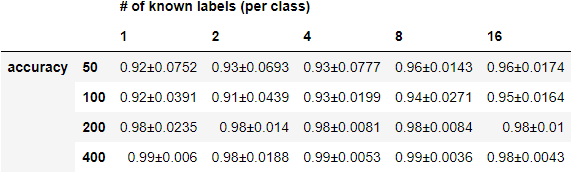
\includegraphics{outputs/part2/laplacian_kernel_interpolation_report.png}

Some observations to make here are:\\


a) Both models seem to perform fairly well, even in the low-data setting.\\

b) Increating the number of known labels increases the accuracy and decreases
 the variance of the predictors.\\

c) Increasing the total number of datapoints generally increases both model accuracies,
and decreases variance. \\

d) The laplacian kernel method outperforms the vanilla inerpolation approach considerably,
on both accuracy and variance. \\


The main reason for the success of this algorithm is the high degree of
 cluster separation observed in the dataset.
\\

For illustration, here is a diagram representing the graph adjacency matrix,
 with colours showing the labelling of an edge. Here blue edges are where both 
labels are -1, teal when both are different, and yellow when both are +1.\\


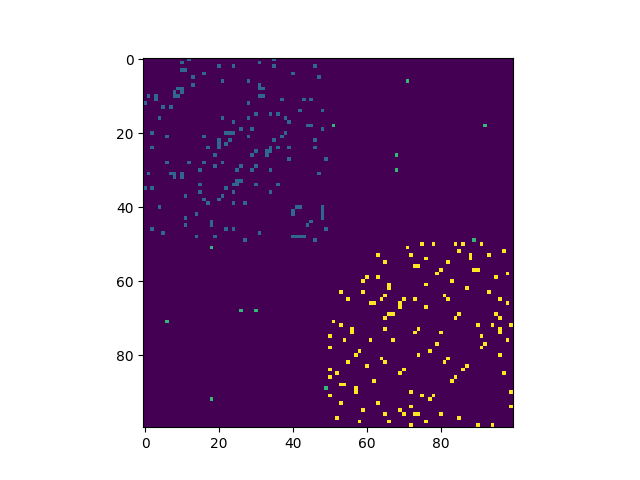
\includegraphics{outputs/part2/graph_label_diagram.png}#

We see through this that the vast majority of datapoints are connected only to points
of the same labelling, and that the graph is highly separated  into 2 clusters.
Hence with minimal training information, both methods are able to predict with a
 high degree of accuracy.\\

Note that error variance decreases as a function of the number of known labels, but 
has a muhc more significant impacgt for the vanilla interpolation method.


We see that the kernel approach consistently outperforms the simple laplacian
 interpolation method. A reasonable explanation for this is that the laplacian
interpolation approach utilises local information to 'diffuse' labels through the graph. 
This means that only datapoints close to labelled data receive information from the 
labels themselves, and accuracy is likely reduced for datapoints far from the labels.
In contrast, the kernel interpolation method takes global information from all the 
labelled datapoints and weights them according to their proximity and connectedness 
to eachother to predict labels.
\newpage



\section{PART III}
\subsection{Questions}
\begin{itemize}
    \item[a.]
    \item[b.]
    \item[c.]
    \item[D.]\\
    We note that since for any $X_{t}$, $y_{t} = X_{1,t}$, we have the following
     expression representing the linear separability of our dataset:\\
    \[(v \cdot x_{t})y_{t} \ge 1\]\\
    Where $v = (1,0, \dots, 0)^{T}$. Note that $\|v\| =1$.\\
    Hence, in our online mistake bound for the perceptron, we have that $\gamma =1$.
    Further note that $\forall t$, $x_{t} \in {-1,1}^{n} \implies \|x_{t}\|^{2}
    = n$. This gives us that $R = max_{t} \|x_{t}\| = \sqrt{n}$.
    Hence our mistake bound for the perceptron algorithm is given by:\\
    
    \[M \le n \].\\

    Using the theorem on page 60 of the online learning notes, we arrive at:\\

    \[Prob(\mathcal{A_{S}}(x ^{\prime}) \ne y^{\prime} ) \le \frac{n}{m}\]\\

     
\end{itemize}
\end{document}
